\chapter{Model}
Należy wpierw stworzyć doskonały model kinematyczny, aby móc porównać z nim stworzony model dynamiczny, oraz fizyczną platformę.
Dzięki temu można łatwo oszacować jak bardzo błędy symulacji, oraz błędy niedoskonałości fizycznego modelu odstają od matematycznych wyliczeń.

Dodatkowo stworzenie platformy kinematycznej pozwalało na porównanie szybkie odrzucanie niedziałających implementacji modelu kinematycznego.
\begin{figure}[H]
\centering
 \includegraphics[width=0.8\textwidth]{graphics/base_dims.pdf}
\caption{Wielkości używane we wzorach.}
\label{fig:base_dims}
\end{figure} 

\begin{table}
\centering
\begin{tabular}{c c l}
Oznaczenie & Wartość & Opis \\
\hline
$r$ & 0,1 m & Promień koła w najszerszym miejscu na środku. \\
$a$ & 0,76 m & Szerokość platformy między środkami kół tej samej osi. \\
$b$ & 0,72 m & Długość platformy między środkami kół tego samego boku. \\
$\omega_i$ & & Prędkość kątowa każdego z kół. \\
$v_x$ & & Prędkość transwersalna w osi X. \\
$v_y$ & & Prędkość transwersalna w osi Y. \\
$\omega_z$ & & Prędkość kątowa w osi Z, wektor skierowany w górę. \\
\end{tabular}
\caption{Opisy i wartości symboli używanych we wzorach i rysunkach.}
\label{tab:dims}
\end{table}


\section{Sposób zapisu w formacie SDF}
\emph{Simulation Description Format} (SDF) jest formatem XML pozwalającym na określenie elementów i zależności pomiędzy nimi w przestrzeni trójwymiarowej, w szczególności budowy i rozmieszczenia robotów.
Powstał jako zamiennik URDF ze względu na jego skomplikowaną semantykę i brak możliwości określania ważnych cech, jak rozmieszczenia elementów na symulowanej scenie, określania materiałów itp.

W przeciwieństwie do poprzednika zapisującego model w przestrzeni drzewiastej, SDF równolegle określa wszystkie składowe modelu, oraz zależności między nimi, jak więzy i względne pozycje.
Standard jest dobrze opisany na ich stronie internetowej \cite{sdf_website}.

Na szczycie wszystkich elementów znajduje się element \texttt{world} zawierający w sobie wszystkie modele na symulowanej scenie.
Mogą być to roboty, a także przeszkody, źródła światła, elementy animowane i tym podobne.
Dodatkowo można dodać informację o ustawieniach maszyny symulującej fizykę, wyglądzie sceny, wietrze, grawitacji, polu magnetycznym i tym podobnych.

W każdym z modeli oznaczonych tagiem \texttt{model} zawiera się nazwa, domyślna pozycja, sposób traktowania przez symulator i wtyczki programów obsługujących zaawansowane zachowanie modelu.
Można przenieść zawartość elementu do innego pliku i określić ścieżkę do importu.

Model ma w sobie równolegle wszystkie elementy oznaczone jako \texttt{link}, każdy z nich jest osobną, kompletną częścią robota, na przykład kołem, fragmentem ramienia chwytaka, trzonem.
Zawiera w sobie informacje o pozycji względem innych obiektów, masie, kształcie, kolizjach, materiale fizycznym i wyglądzie.
Pozwala na dodanie do siebie źródeł dźwięku, czujników, baterii itp.

Same elementy zawierają jedynie informacje o swoim początkowym umiejscowieniu w modelu, ale nie o sposobie poruszania się i nałożonych więzach.
Do tego potrzebne są równoległe do elementów modelu typy \texttt{joint} określające typ więzów, osie, współczynniki sprężystości, wytrzymałość, siłę silników.
Każde połączenie określa między jakimi obiektami się łączy.

\section{Model kinematyczny}
Model jest sterowany funkcjami matematycznymi zamieniającymi prędkość ruchu kół platformy na prędkości geometrycznego środka platformy w układzie współrzędnych lokalnych oraz prędkość kątową.
Te funkcje najwygodniej zapisać w postaci macierzowej tak, jak w \cite{wheels}. Wzór powtarza się w wielu innych pracach naukowych, a jego dokładny kształt zależy od kolejności numerowania kół i interpretacji wymiarów.
Dla naszego przypadku:
\[
 \begin{bmatrix}
  v_x \\
  v_y \\
  \omega_z \\
 \end{bmatrix}
 =
 \frac{r}{4}
 \begin{bmatrix}
  -1 & 1 & -1 & 1 \\
  1 & 1 & 1 & 1 \\
  \frac{2}{a+b} & \frac{-2}{a+b} & \frac{-2}{a+b} & \frac{2}{a+b} \\
 \end{bmatrix}
\begin{bmatrix}
 \omega_1 \\
 \omega_2 \\
 \omega_3 \\
 \omega_4 \\
\end{bmatrix}
\]

Uzyskane wartości należy przemnożyć przez odpowiednie wektory jednostkowe, obrócić względem lokalnego układu współrzędnych dla modelu i zastosować w funkcjach nadających prędkości bryle.

Ponieważ sterowanie pozycją modelu kinematycznego odbywa się wyłącznie poprzez wzory matematyczne, w jego symulacji nie uczestniczy maszyna symulacyjna.
Taki model nie reaguje na kolizje z innymi obiektami, nie reaguje na różnicę terenu i nie używa informacji o współczynnikach tarcia materiałów.

W kodzie nadano mu nazwę \texttt{pseudovelma} co odnosi się do tego, że jest to nieprawdziwy ruch sterowany z zewnątrz, a nie prawdziwa symulacja.

\subsection{Problemy implementacji}
Gazebo nie ma zaimplementowanego pełnego wsparcia dla standardu SDF.
W szczególności nie działa struktura elementów \texttt{frame} odpowiadająca za transformacje obiektów względem innych obiektów.
Nie jest to zapisane w dokumentacji, a jedynie zgłoszone od kilku lat w systemie kontroli wersji jako błędy.

Oznacza to, że wszystkie elementy typu \texttt{link} będąc dziećmi \texttt{model} nie przestrzegają jego pozycji.
Powoduje to, że nadając prędkość kątową modelowi za pomocą funkcji nadajemy ją każdemu obiektowi osobno.
Każde z kół i dwie części bazy obracają się zgodnie z zadanymi wartościami, ale ich środki pozostają w miejscu w którym rozpoczęły symulację ignorując kompletnie pozycję w elemencie rodzica \texttt{model}.

Aby to naprawić, należy przenieść zawartość elementów \texttt{link} i ustawić je jako \texttt{visual} tagu \texttt{model}.
W ten sposób traktowane są jako część renderowana modelu, a nie osobne składowe.

Powstała niedogodność jest taka, że ciężej jest sterować obrotem elementów \texttt{visual} i nie można sterować obrotem kół.
Oczywiście ma to znaczenie jedynie kosmetyczne, gdyż w żaden sposób nie wpływa na ruch modelu bazy.

\subsection{Komunikacja}
Komunikacja programu sterującego platformą odbywa się przez wbudowane z ROSa narzędzie \emph{topic}.

Wiadomość o nowych zadanych prędkościach kół nie mieści się w standardzie, zatem został stworzony własny typ \texttt{pseudovelma/Vels}.
Zawiera cztery wartości zmiennoprzecinkowe podwójnej precyzji.
Wartości oznaczają prędkości w rad/s.

Program posiada komunikację:
\begin{itemize}
 \item Nadawanie w każdym cyklu symulacji wiadomości typu \texttt{geometry\_msgs/Pose} z aktualną pozycją i rotacją platformy.
 \item Odbiór wiadomości własnego typu \texttt{pseudovelma/Vels} z zadanymi prędkościami kół.
\end{itemize}

\subsection{Zachowanie}
Platforma ignoruje kompletnie otoczenie poruszając się przez inne obiekty.
Po nadaniu stałych prędkości kół następuje ruch po okręgach zgodnie z przewidywaniami.

Cały czas zwraca aktualną pozycję i rotację działając jak układ całkujący funkcje ruchu z powyższej macierzy.

\section{Model dynamiczny}
Wykorzystując maszynę do symulacji fizyki możemy umieścić w niej model określający kształty, masy i zależności obiektów, potem nadać elementom wirtualny ruch i otrzymać przybliżone wyniki do tego, jak zachowywałaby się rzeczywista platforma.

Wszystkie elementy związane z tym modelem noszą nazwę \texttt{omnivelma}, co nawiązuje do wielokierunkowości ruchów robota manipulującego którego podstawa ma transportować.

Robot jest bryłą na którą składają się następujące części składowe:
\begin{itemize}
 \item Główna część trzonu.
 \item Ruchoma, mniejsza część trzonu z przodu robota.
 \item 4 koła, 2 podłączone do głównej części, a 2 do przedniej.
 \item Po 12 rolek na każdym kole.
 \item Przegub zawiasowy łączący dwie części podstawy.
 \item 4 przeguby zawiasowe z silnikami łączące części bazy z kołami.
 \item 12 przegubów zawiasowych na każdym kole łączących koła z rolkami.
\end{itemize}

Jak widać jest dość skomplikowany obiekt do symulacji, dlatego bezpośrednie podejście poprzez budowę modelu jak najdoskonalszego oryginałowi można wykluczyć.
Powodowałaby olbrzymią ilość obliczeń maszyny symulacyjnej, każde obarczone błędem.

Istnieją różne podejścia do stworzenia odpowiedniego modelu. Każde z nich było proponowane na różnorakich forach przez osoby symulujące podobne bazy.
Jednak rozwiązanie nigdy nie zostało znalezione.
Działający w naszym przypadku sposób także nie został wcześniej sprawdzony.

\subsection{Jak największe zbliżenie do oryginału}
Wspomniany wyżej sposób jest najbardziej wymagającym obliczeniowo, ale także najprostszym z możliwych.
Wystarczy stworzyć elementy i nadać im fizyczny kształt za pomocą odpowiedniej siatki trójkątów.
Kształt może być także nadany poprzez przybliżenie jedną z podstawowych brył, jak sześcian, kula, łamana, walec i płaszczyzna.
Takie przybliżenie znacznie przyspiesza obliczenia, gdyż może być specjalnie traktowane przez algorytmy.

Słabym punktem tego rozwiązania jest fakt, że rolki są niestandardowym kształtem, którego dokładność jest bardzo wysoce wymagana.
Przybliżenie jej walcem powoduje problemy przy przenoszeniu ciężaru na kolejną rolkę, gdyż koło będzie musiało przez chwilę oprzeć się o krawędź.
Taki model naturalnie podskakiwałby przy ruchu zwiększając tym samym i tak duże niedokładności.

Przybliżenie rolki siatką jedynie zmniejsza powyższy efekt, gdyż sama siatka zbudowana jest z prostych odcinków.
Zwiększając jej gęstość zwiększamy jakość symulacji, ale narażamy się na olbrzymi skok ilości obliczeń.
Kalkulowanie kolizji z siatką jest najdroższe z możliwych.

\subsection{Resetowanie pozycji koła}
Ten sposób został użyty w modelach w symulatorze V-Rep.

Polega on na tym, że koło podłączone do bazy posiada przegub zawiasowy obrócony pod kątem 45\textdegree, tak aby był równolegle do dolnej rolki.
Do tego przegubu podłączona jest kula reagująca z podłożem, którą to w każdej iteracji symulacji resetujemy do pozycji wyjściowej razem z przegubem.

\begin{easylist}[itemize]
\ListProperties(Style*=--- )
& Trzon całego robota.
& Przegub zawiasowy z silnikiem, któremu nadajemy odpowiednią prędkość.
&& Wirtualne koło łączące ze sobą dwa przeguby. Obraca się tak samo, jak obracało by się rzeczywiste koło.
&&& Siatka powodująca ładny wygląd koła i pozwalająca na łatwe stwierdzenie jego rotacji.
&&& Wewnętrzny przegub zawiasowy obrócony o 45\textdegree w stosunku do osi koła. Pozycja i rotacja tego przegubu jest resetowana do pozycji początkowej względem trzonu po każdej iteracji maszyny symulacji.
&&&& Kolizja koła w formie kuli, symuluje aktualnie najniższą rolkę u podłoża. Jego pozycja i rotacja są resetowane po każdej iteracji do pozycji początkowej względem trzonu podstawy.
\end{easylist}

Wywołuje to takie działanie, jak gdyby na kole istniała jedynie dolna rolka. Przez krótką chwilę model zachowuje się poprawnie, aż obrót drugiej osi zacznie wpływać na symulację.
Zanim to jednak nastąpi, jego rotacja jest przywracana do pozycji początkowej.
Ponieważ robimy to natychmiast, maszyna symulacyjna nie bierze pod uwagę tarcia i ruchu w takim przypadku.

Niestety nie jest możliwe uzyskanie tego rozwiązania w Gazebo, gdyż struktura drzewiasta obiektów nie jest zaimplementowana.
Metody zmieniające pozycję obiektu nie działają.
W dodatku potrzebna jest także możliwość ustawiania rotacji i pozycji przegubu, elementu \texttt{joint}, co nie jest wystawione do modyfikacji w API.

Bardzo skomplikowany sposób działania kół skłania do szukania innych rozwiązań.

\subsection{Zmiana osi rolki}
Poprzedni przypadek można zmodyfikować poprzez wyznaczanie nowej osi przegubu łączącego wirtualne koło z kulą symulującą rolkę.

Oś wewnętrzna podłączona jest do koła wirtualnego i obraca się razem z nim.
W każdym cyklu należy zamienić obróconą już nieco oś na kierunek pierwotny względem postawy platformy.
Spowoduje to, że kolejna iteracja fizyki będzie mogła obracać kulą reprezentującą rolkę pod odpowiednim kątem.

Należało obliczyć kierunek w przestrzeni globalnej biorąc pod uwagę aktualną pozycję platformy i obrót kół.
Fakt, że program wymagał wektora relatywnie do pozycji koła wirtualnego bardzo komplikował obliczenia.

Trzeba było jeszcze wybrać moment wyznaczenia nowego kierunku osi, bowiem maszyna symulacyjna wywołuje wiele różnych funkcji w jednym cyklu symulacyjnym.
Można wywołać kod w różnych momentach z teoretycznie różnym efektem. 

Implementacja tego rozwiązania niestety nie stworzyła działającego modelu.
Wykonywanie kodu w różnych momentach symulacji nie wpływało na efekt.
Platforma poprawnie poruszała się do przodu i do tyłu. 
Pierwszy problem pojawiał się gdy w czasie ruchu na bok, prędkość malała, aby zmienić zwrot pomimo niezmiennej prędkości kół.
Po kilku sekundach problem się powtarzał.

Drugim problemem był ruch po krzywej w której model nieregularnie podskakiwał w końcu nawet obracając się w pionie.
Takie zachowanie oczywiście dalekie jest od oryginału.

Wygląda na to, że problemem było wewnętrzne traktowanie przegubów przez maszynę symulacyjną.
Takie nienaturalne zachowanie jak nagła zmiana osi przegubu musiała wprowadzać nieprawdopodobne wartości do zmiennych stanu, co w rezultacie powodowało po pewnym czasie chaotyczny ruch.

\subsection{Modyfikacja kierunków i wartości wektorów tarcia}
Warto tu wytłumaczyć, w jaki sposób maszyny symulacji fizyki interpretują kolizję i dotyk.

\begin{figure}[H]
\centering
 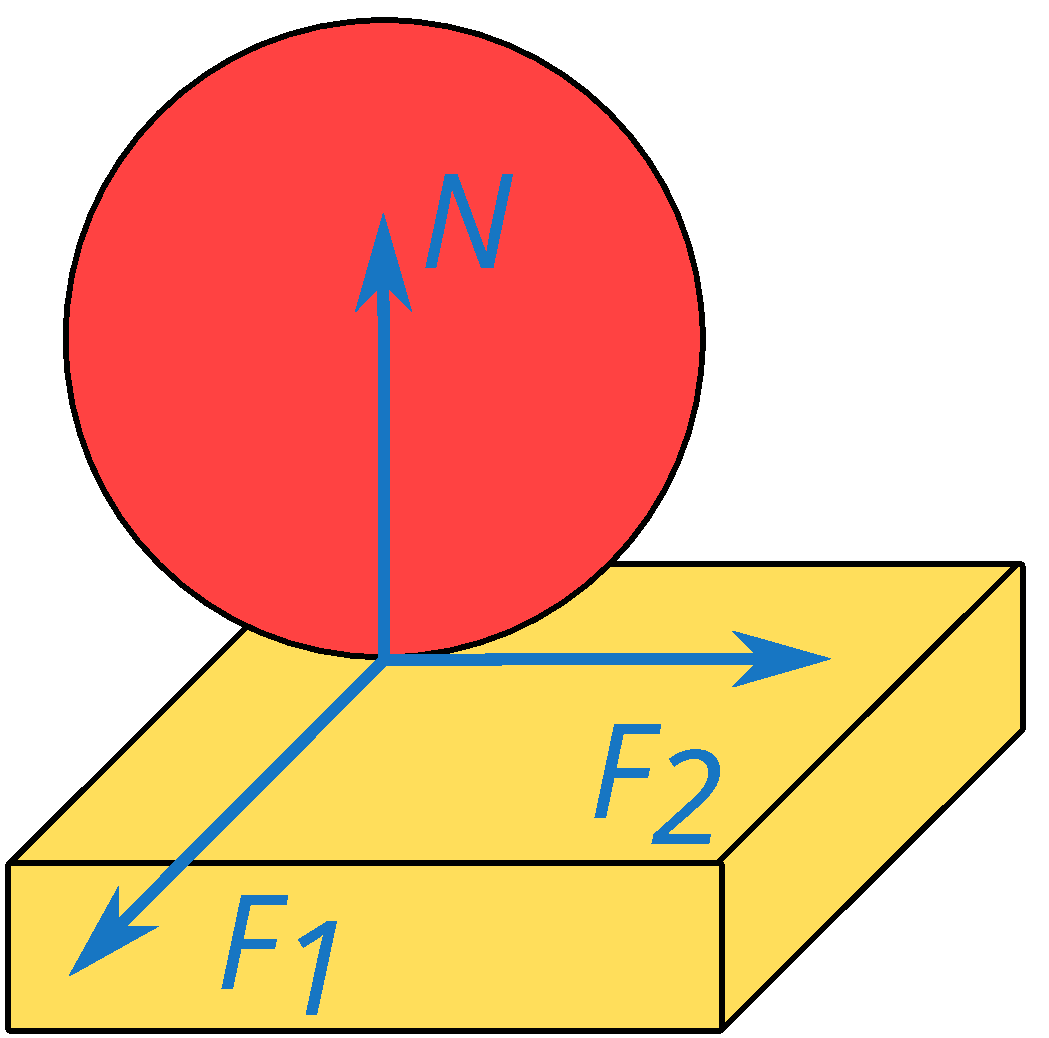
\includegraphics[width=0.5\textwidth]{graphics/friction.pdf}
\caption{Wektory punktu kolizji.}
\end{figure} 

Po wykryciu punktu kolizji i wyznaczeniu wektora normalnych $N$ do dotykających się obiektów należy zadziałać odpowiednimi siłami, aby zatrzymać, lub odbić obiekty.
Dodatkowo ponieważ prędkości obiektów nie muszą być równoległe do wektora kolizji, należy zasymulować siłę tarcia z odpowiednią dla współczynnika tarcia wartością.
Można to uzyskać nadając punktowi siłę prostopadłą do wektora normalnych, ten wektor może być rozpisany przy pomocy dwóch wektorów jednostkowych $F_1$ i $F_2$. 
Te wektory są prostopadłe do wektora normalnych, równoległe do płaszczyzny kolizji.

W normalnej symulacji nigdy nie potrzeba osobno modyfikować współczynników tarcia wzdłuż tych wektorów, gdyż powierzchnie obiektów mają równe współczynniki tarcia w każdym kierunku.
Jednakże modyfikując je statycznie, lub dynamicznie można uzyskać bardzo ciekawe efekty.
Instrukcja podaje przykład w którym, aby zamodelować tarcie opon samochodu prostopadle do kierunku jazdy, należy dynamicznie zmieniać współczynnik tarcia dla wektora $F_1$, lub $F_2$ w tym kierunku.
Współczynnik tarcia prostopadle do kierunku jazdy może być liniowo zależny od prędkości.
Spowoduje to, że im większa prędkość samochodu, tym boczna siła łatwiej zmieni tor jego jazdy, co ma odwzorowanie w rzeczywistości.
Więcej informacji można znaleźć na stronie instrukcji maszyny symulacyjnej ODE \cite{ode_contact}.

W naszym modelu modyfikujemy kierunek wektora $F_1$, oraz współczynniki tarcia w obu kierunkach, aby przybliżyć zachowanie się rolki.
Ponieważ wektory $F_1$ i $F_2$ są określone w globalnym układzie współrzędnych, w każdej iteracji maszyny symulacji należy obrócić je względem aktualnej pozycji bazy.
W doskonałym przypadku rolka obraca się całkowicie bez tarcia, a ruch wzdłuż jej osi jest niemożliwy.
Można więc ustawić zerowy współczynnik tarcia w kierunku prostopadłym do osi, oraz nieskończenie duży dla wektora równoległego do osi.

\begin{figure}[H]
\centering
 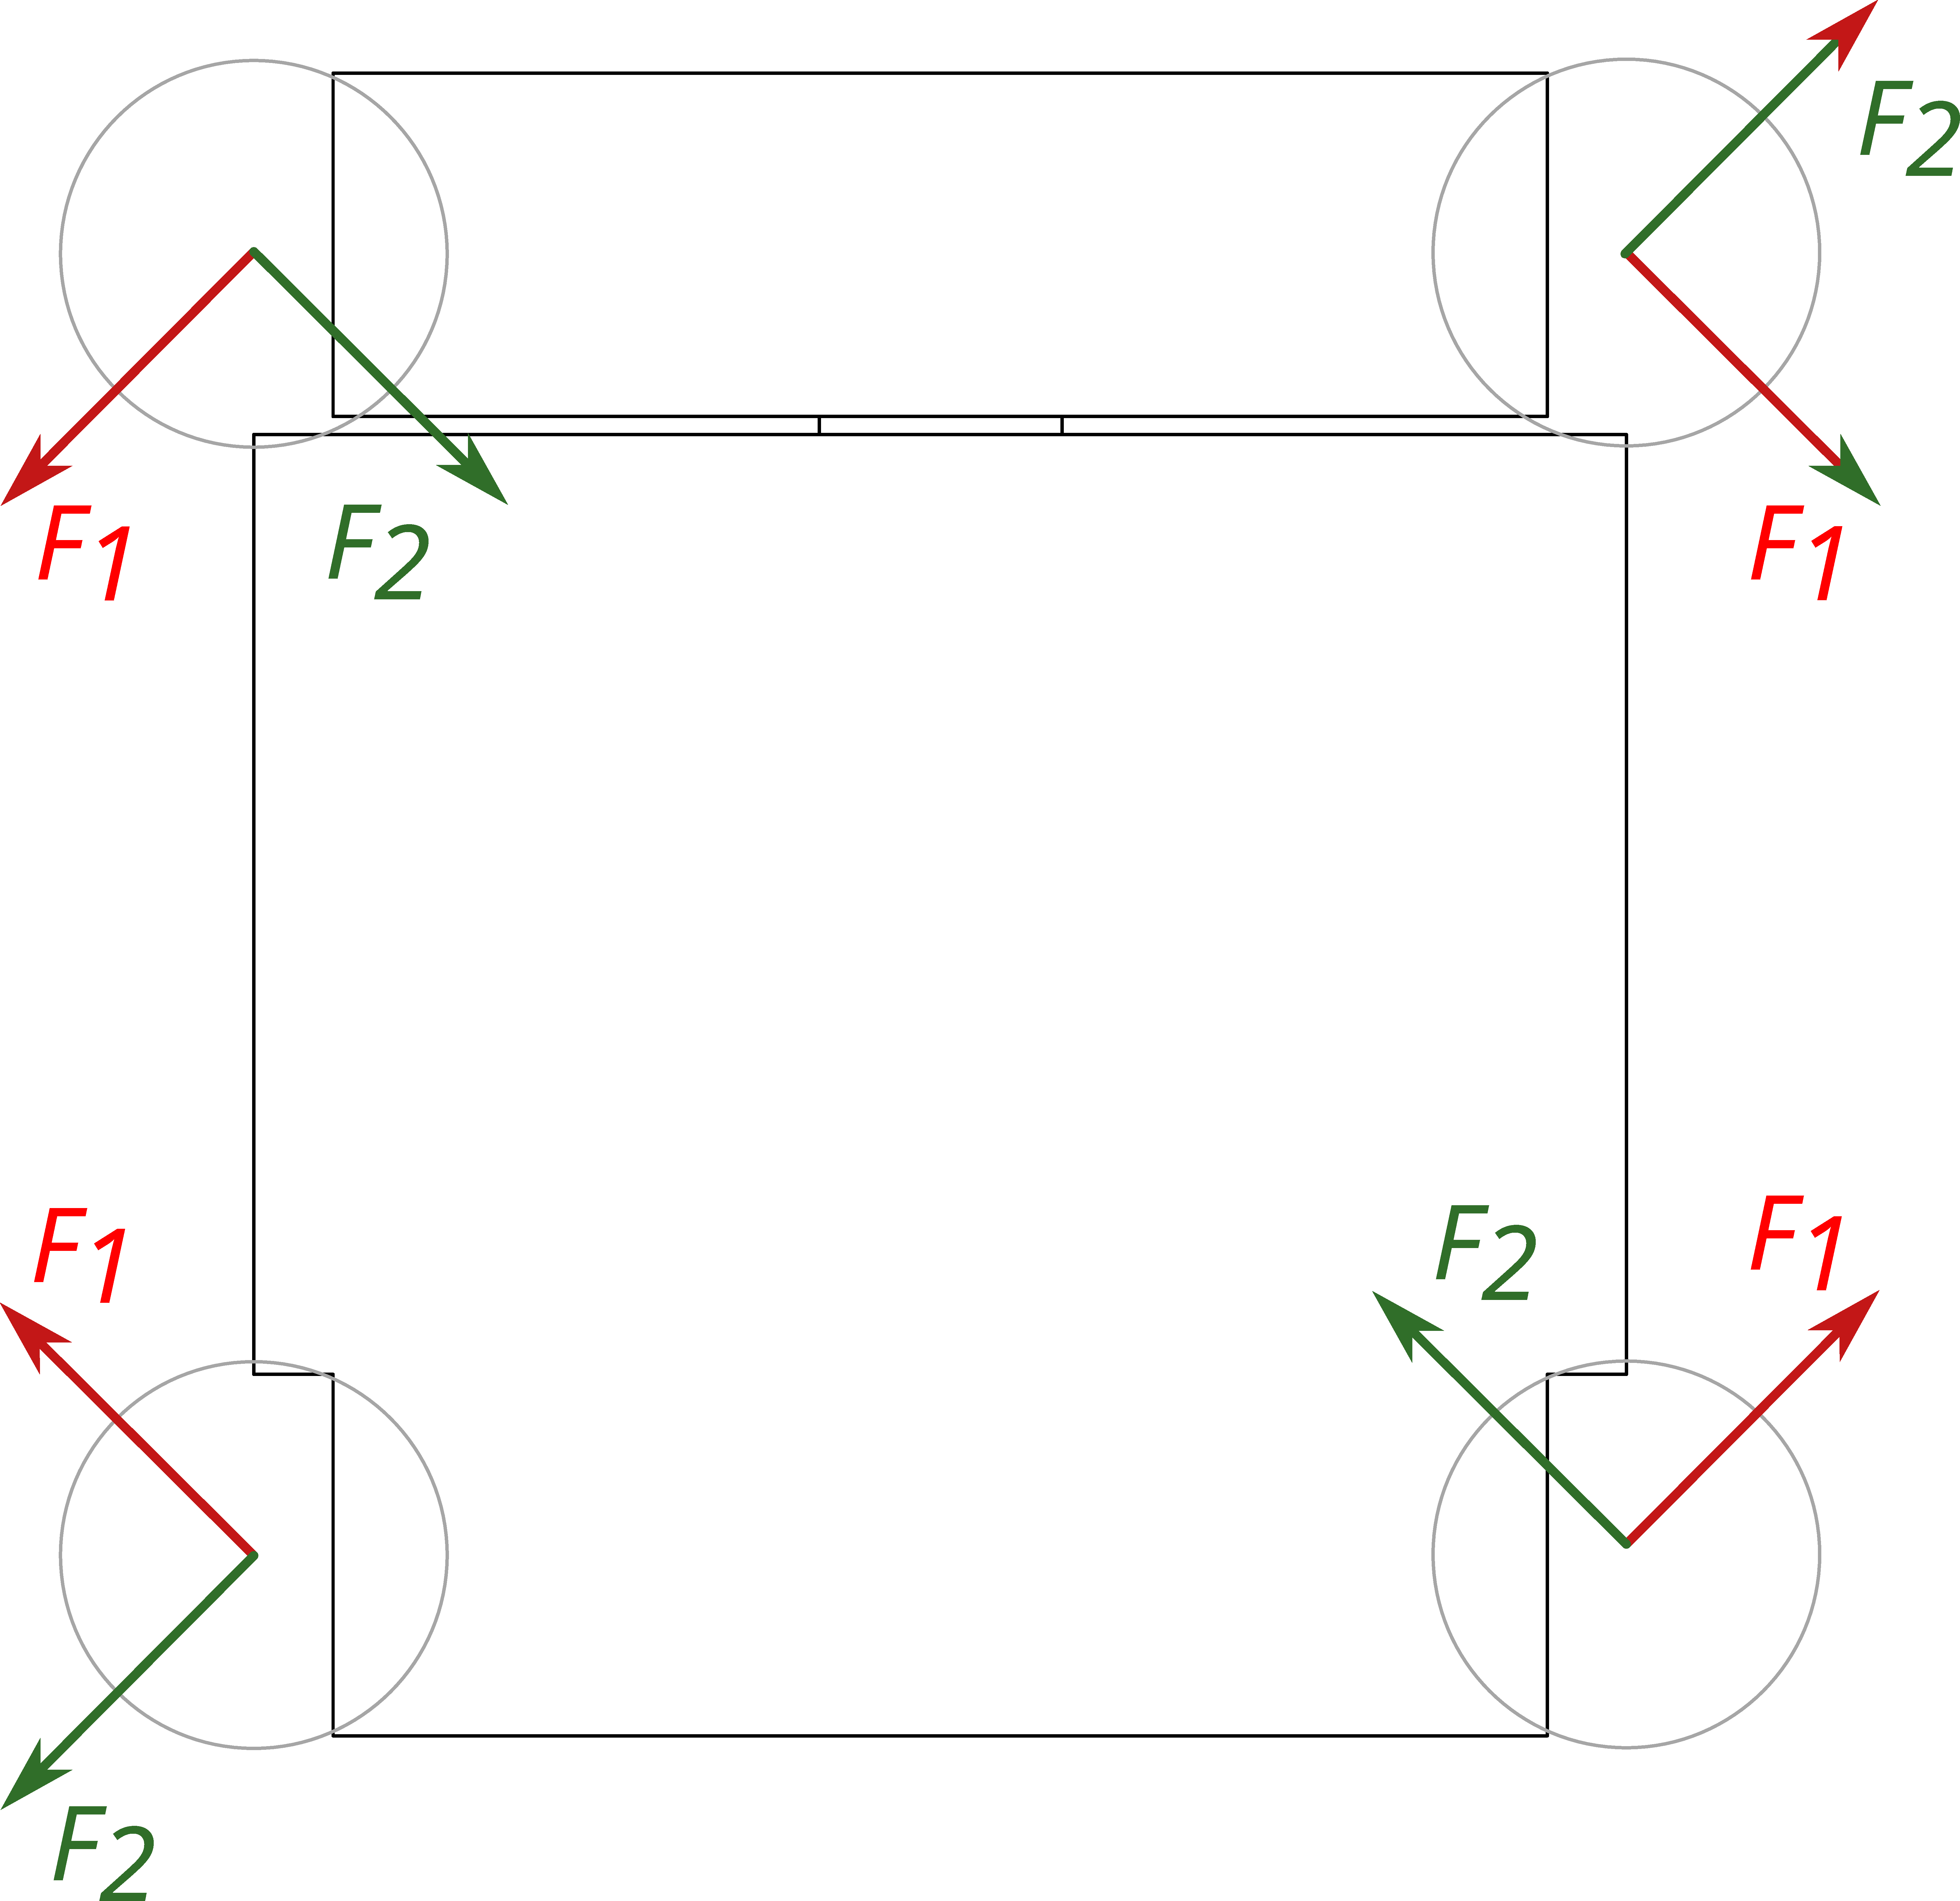
\includegraphics[width=0.8\textwidth]{graphics/base_vects.pdf}
\caption{Kierunki wektorów dla których należy nadać współczynniki tarcia przy symulacji platformy. Tarcie w kierunku $F_1$ powinno być nieskończone, a w $F_2$ zerowe.}
\end{figure} 

Niestety w rzeczywistości rolki wykonane są ze śliskiego plastiku, który pozwala na mały ruch wzdłuż ich osi.
Osie kolek również nie obracają się płynnie, trzeba użyć dużej siły, aby obrócić każdą z nich, pod naciskiem platformy tarcie jest jeszcze większe.
Każda rolka w dodatku obraca się z innym tarciem wprowadzając kolejne zakłócenia.
Podłoże także nie jest tu bez znaczenia.
Należy zatem wystawić interfejs do łatwej zmiany współczynników tarcia, aby później dobierać odpowiednie wartości na podstawie zachowania rzeczywistego robota.

Podobnie, jak w poprzednich przypadkach modelujemy tylko najniższą, dotykającą podłoża rolkę.
Jak wcześniej wspomniano, ma ona bardzo skomplikowany kształt, lecz można przybliżyć całe koło kulą.
Mamy zatem w miejscu każdego koła po jednej kuli z dynamicznie modyfikowanym tarciem i ładną siatką w kształcie koła, oraz przegub z motorem łączący odpowiednią część bazy z kołem.
To najprostsza budowa modelu (a zatem najszybsza) z poprzednich.

Takie rozwiązanie wiąże się z pewnym ryzykiem.
Wymaga, aby symulator używał maszyny ODE, co zmniejsza przenośność modelu. ODE jest domyślnym symulatorem w Gazebo.
Maszyna Bullet również liczy kolizje w ten sposób i ma modyfikowalne wektory, lecz nie daje podobnych wyników. Być może jest to spowodowane brakiem odpowiedniej konfiguracji.

\subsection{Komunikacja}
Ze względu na wiele ustawień elementów bazy, należy stworzyć bogaty interfejs.
\begin{itemize}
 \item Nadawanie w każdym cyklu symulacji wiadomości typu \texttt{geometry\_msgs/Pose} z aktualną pozycją i rotacją platformy.
 \item Odbiór wiadomości własnego typu \texttt{pseudovelma/Vels} z zadanymi prędkościami kół.
 \item Odbiór wywołań ustawiających współczynniki tarcia wzdłuż wektorów $F_1$ i $F_2$.
 \item Symulator enkodera nadający aktualną pozycję i rotację obiektu.
 \item Odbiór wywołań ustawiających masy i momenty obrotowe niektórych elementów składowych konstrukcji, oraz masy transportowanego robota.
\end{itemize}

\section{Porównanie modeli}
Posiadając model kinematyczny, którego ruch jest sterowany wzorami możemy porównać jego pozycję i rotację z modelem dynamicznym.
Należy w tym samym momencie nadać bazom identyczne prędkości kół i zbierać dane dotyczące wzajemnej pozycji.
Nadano kołom kolejne prędkości zgodnie z numeracją w rysunku \ref{graphics:base_dims}, $(-2 , 1 , 0 , -3)$.

\begin{figure}[H]
\centering
 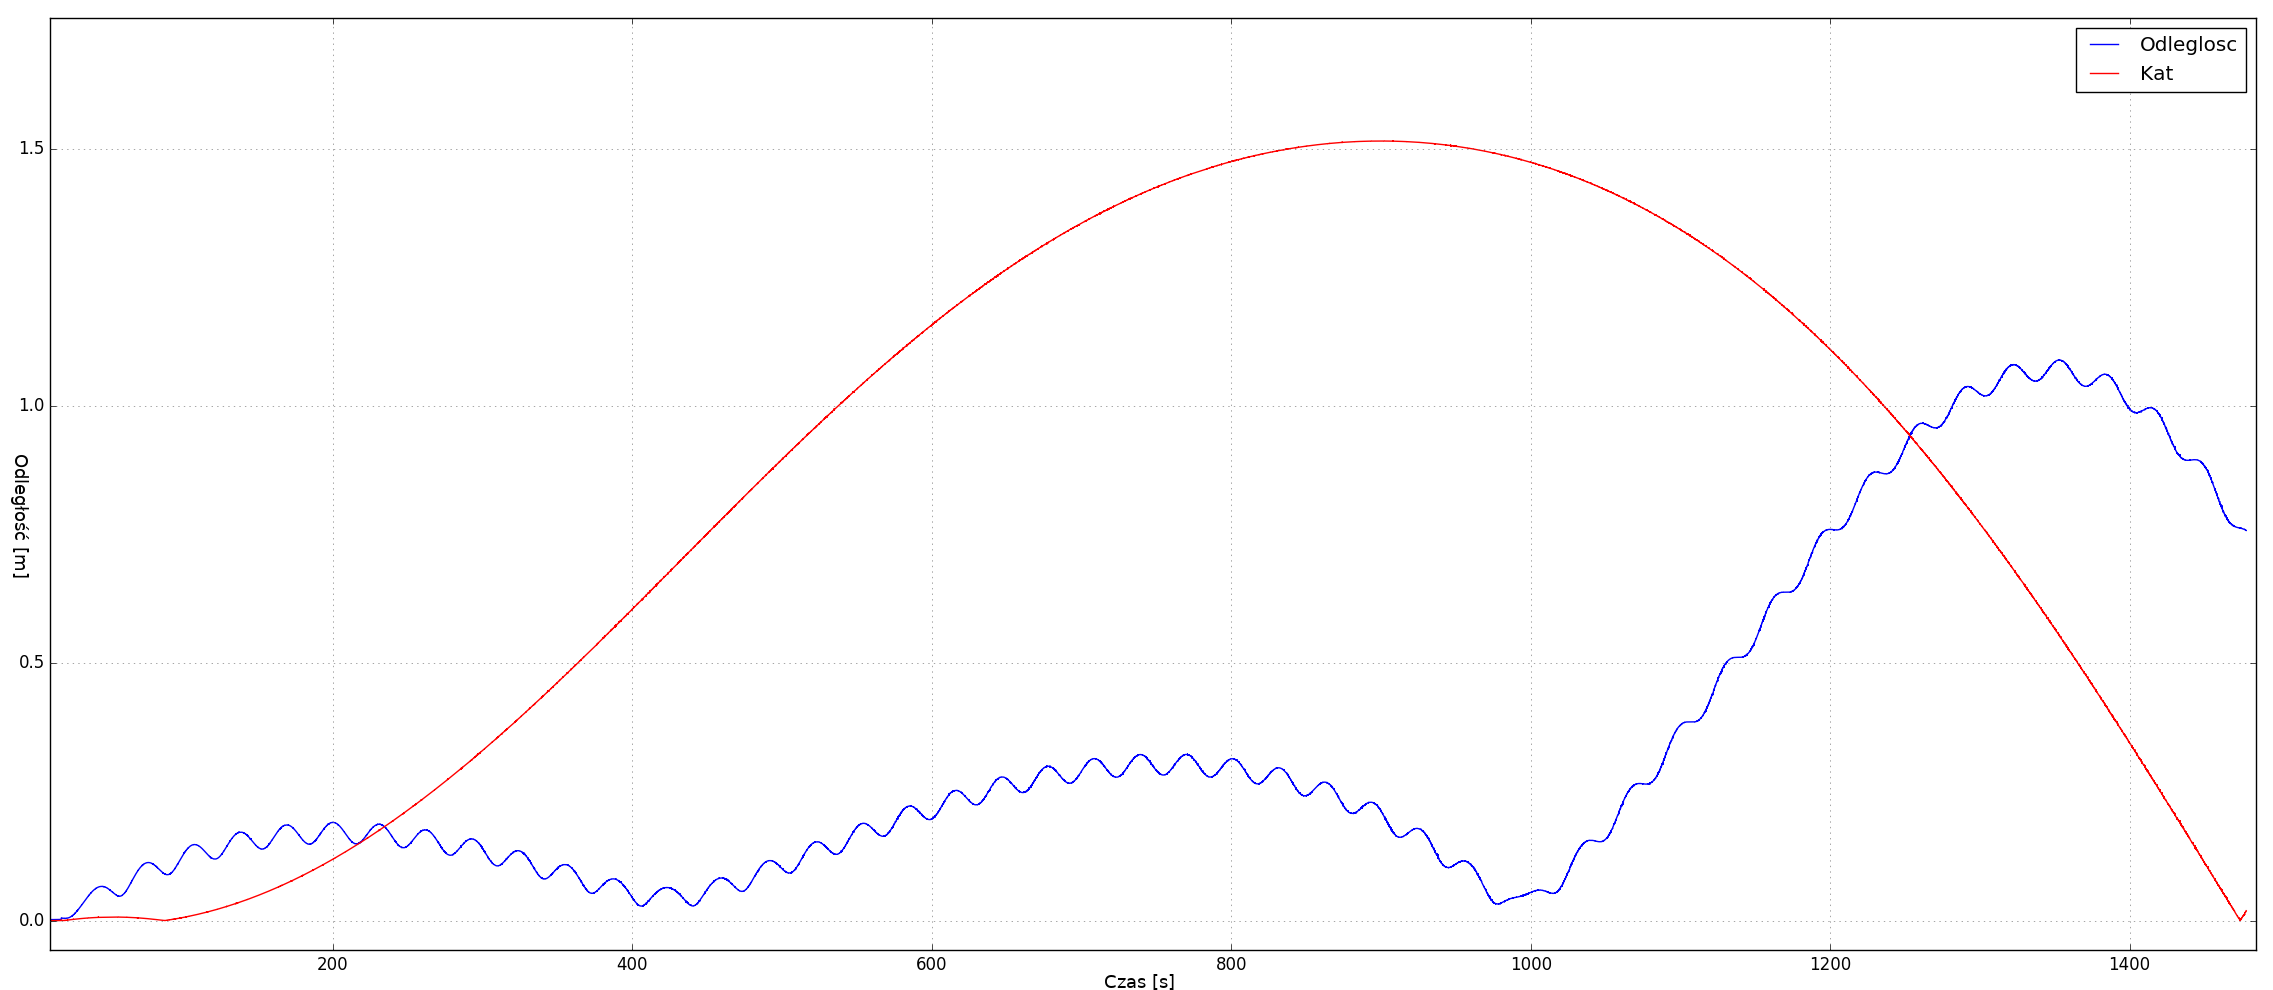
\includegraphics[width=\textwidth]{graphics/test1.png}
\caption{Odległość i kąt pomiędzy platformami w czasie.}
\end{figure} 

Takie ustawienie spowodowało ruch po okręgu o okresie ok. 32 s.
Modele początkowo posiadały zbliżoną pozycję i rotację, ale w miarę upływu czasu opóźnienia modelu dynamicznego stały się zauważalne.
Także kąt między nimi zaczął się zmieniać, lecz w znacznie większym stopniu, niż wynikałoby to z opóźnienia pozycji.
Przez cały czas trwania eksperymentu model dynamiczny zrobił kąt pełny w stosunku do kinematycznego, a jego odległość zmieniała się sinusoidalnie.
Oba modele wykonały tę samą ilość obiegów.

Po pierwsze widać, że już na samym początku pomiarów odległość nagle wzrosła, co jest spowodowane poślizgiem platformy przy nadaniu kołom prędkości.
Model kinematyczny rozpoczyna jazdę natychmiastowo.
Dzieje się tak pomimo doskonałym współczynnikom tarcia, w dodatku masa platformy nie jest dobrana zgodnie z rzeczywistością.
Ten efekt może być zmniejszony za pomocą ustawiania współczynnika tarcia podłoża, ale nie jest możliwe jego całkowite wyeliminowanie, gdyż jest to cecha maszyn symulacji fizyki.

Drugą zauważalną cechą wykresu są małe oscylacje o okresie jednego obiegu.
Ma to efekt taki sam, jak gdyby obie platformy wystartowały z różnych pozycji, których odległość jest mniejsza od średnicy trasy.
To powodowałby, że odległość między ich pozycjami oscylowałaby w właśnie taki sposób.
Modele wystartowały z tego samego punktu w tym samym czasie, jednakże środek ciężkości modelu dynamicznego nie pokrywał się ze środkiem platformy względem którego obliczano pozycję.
W związku z tym jej ruch odbywa się wokół środka ciężkości masy, ale pozycja jest liczona względem geometrycznego środka.
To pokazuje, że należy bardzo dokładnie ustawić masy elementów składowych w stosunku do rzeczywistego modelu, gdyż w przeciwnym wypadku symulacja obarczona będzie właśnie takimi oscylacjami.
Co więcej, ruchome elementy transportowanego robota manipulującego będą miały wpływ na pozycję środka ciężkości i ruch podstawy.
Dlatego należy wprowadzić element transportowanej masy, którego środek ciężkości powinien być modyfikowalny.

Trzecią cechą są duże oscylacje, rosnące w czasie.
Na razie nie jest dokładnie wiadome, dlaczego powstają.
Warto jednak zauważyć, że nie są zbieżne w czasie z kątem obrotu, gdyż jego wartość ma mniejszy okres.

Opóźnienia powstałe na modelu dynamicznym są cechą dokładności maszyny symulacyjnej fizyki i nie da się ich całkowicie wyeliminować.
Jednakże ich wartość jest znacznie mniejsza od niedokładności wprowadzonej przez niedoskonałość rzeczywistego obiektu.
To oznacza, że model ma rzeczywistą wartość pod kątem pomocy w symulacji robota.

\section{Podsumowanie}
W kolejnych przygotowaniach do pracy udało się przetestować różne sposoby modelowania bazy, znaleźć najlepszy działający i stworzyć modele.
Porównanie działania modelu z wartościami obliczonymi matematycznie pozwoliło zobaczyć możliwe problemy, które pojawią się we współpracy z rzeczywistą platformą.

Została zdobyta wiedza na temat problemów obsługi programu Gazebo, oraz jego integracji z ROSem, jakie funkcjonalności nie są zaimplementowane i jakie nie działają.
Nie jest to nigdzie dobrze opisane, więc błędy zdarzały się w zupełnie nieprzewidzianych okolicznościach.

Należało nauczyć się działania architektury systemu ROS, aby poznać działanie jego składowych i obsługę standardowych programów.
Udało się uzyskać standardowe pakiety systemu ROS kompilowane przez jego systemy, komunikujące się w standardowy sposób i przenośne na inne komputery.
Tutaj również pojawiły się niestandardowe problemy z kompilacją, na przykład zła kolejność generacji plików rozwiązywalna przez zresetowanie systemu operacyjnego.

Należy teraz stworzyć identyczny model w programie V-Rep, a dokładniej zmodyfikować istniejący Kuka Youbot pod kątem rozmiarów bazy.
Trzeba go podłączyć do systemu ROS w taki sam sposób, jak poprzednie, aby dało się nim równie łatwo sterować.

Należy dodać dużą ilość interfejsów do zmiany różnych parametrów modelu, między innymi masy, moment obrotowy, transponowana masa i jej środek ciężkości.
Platforma musi zwracać wartości enkodera jak pozycja i prędkość.
Warto dodać elementy dodatkowe, jak model interaktywnego podłoża ze zmiennym współczynnikiem tarcia.

Do zrobienia jest także system ułatwiający manualne sterowanie bazą za pomocą interfejsu graficznego i zbierający informacje do porównania z ruchami prawdziwego robota.
Interfejs graficzny będzie wtyczką w QT tworzącą kolejny panel w ROSowym programie \emph{rqt}.

Na koniec używając wystawionego interfejsu metodą prób i błędów należy znaleźć takie ustawienia (np. masa, tarcie), które produkują rezultat najbardziej zbliżony do działania rzeczywistego modelu.
Ten zabieg może trwać nieokreśloną ilość czasu, a wpływ na niego będzie miał stan modelu robota manipulującego i pozostałe elementy składowe.
